\documentclass[11pt,a4paper]{article}
\usepackage[margin=2.2cm]{geometry}
\usepackage{amsmath,booktabs,tikz}
\usepackage[hidelinks]{hyperref}
\usetikzlibrary{arrows.meta,positioning}
\title{\texttt{RankIncidence} over a scalar type parameter}
\author{Plan 2026-10-20-rank-incidence-scalar (branch \texttt{feat/rank-incidence-scalar})}
\date{Created-at 2026-10-20 03:01 CEST}
\begin{document}
\sloppy
\maketitle
\paragraph{Directive.} User, 2026-10-20 02:5x, after ``why reduce to CSR at all -- could it be a view, converted
quickly from a general representation?'': ``feat branchen bevihetj\"uk''. \texttt{hymeko\_graph} is an item of this
repository's \texttt{CORE.YAML}; this plan is the written justification its \S1 asks for, and the branch is the
user's chosen vehicle. Nothing is merged or pushed without a further instruction.

\paragraph{Why.} The cell rank is already the zero-conversion view a CSR would copy: row $r$ is
\texttt{members[r$\cdot$k..(r+1)$\cdot$k]}, \texttt{RankCofaces} its transpose. P28/P30 (Nagare, 2026-09-26) measured
it 11--16$\times$ faster to build and 2.4--4.2$\times$ faster to reverse than CSR. A consumer that needs \texttt{f64}
-- the one-form normal operator of \texttt{nagare\_autoholonomy}, whose solvers run in \texttt{f64} -- cannot use the
view, since every value table and kernel is \texttt{f32}; so it assembled a CSR instead. The fix is the scalar, not a
second view.

\paragraph{ETA.} 2\,h: the trait and the generic view 1\,h, the gates (this crate, Nagare's suites through a local
\texttt{[patch]}) 1\,h.

\section{Design}
\begin{itemize}
\item \texttt{pub trait IncidenceScalar: Copy + Send + Sync + Debug + PartialEq + Add + Mul + Neg + AddAssign +
  MulAssign \{ const ZERO; const ONE; fn from\_count(usize) -> Self \}}, implemented for \texttt{f32} and \texttt{f64}.
\item \texttt{RankIncidence<'a, F: IncidenceScalar = f32>} and \texttt{Signs<'a, F = f32>}: the value tables, the
  kernels (\texttt{lower\_to\_cell}, \texttt{cell\_to\_lower} and their adjoints, the sign gradients) and the private
  \texttt{SignLookup}, \texttt{accumulate}, \texttt{dot} over \texttt{F}. The bit-packed $\pm1$ signs yield
  $\pm$\texttt{ONE}, the same bits the \texttt{f32} bit trick produced.
\item \texttt{CellTopology} keeps \texttt{f32} storage; \texttt{incidence} returns \texttt{RankIncidence<'\_, f32>}.
  The default parameter keeps every existing use -- \texttt{hyper\_operator}, Nagare's \texttt{hg\_message},
  \texttt{hypergraph\_conv}, \texttt{differentiable} -- compiling unchanged.
\end{itemize}
\section{Contracts}
\begin{itemize}
\item \textbf{Bit identity of the \texttt{f32} path}: every expression keeps its order; \texttt{1/k} is
  \texttt{ONE / from\_count(k)}, the same \texttt{f32}. Gates: this crate's suite, and Nagare's common/core/vision
  suites (hundreds of HSiKAN bit pins) built against this branch.
\item \textbf{New tests}: the \texttt{f64} view against the \texttt{f32} one on exactly representable data, and
  against a dense reference; adjoint identities $\langle Bx, y\rangle = \langle x, B^{\mathsf T}y\rangle$ in
  \texttt{f64}.
\item \textbf{Out of scope here}: the forward-kernel speed gap P28 found; it is the next item on this branch, gated on
  a quiet criterion A/B.
\item \textbf{Rollback}: the branch.
\end{itemize}
\section{Amendment 1 (2026-10-20 03:41 CEST): the kernel gap, first step}
\begin{itemize}
\item \textbf{Row width as a type parameter.} The kernels take \texttt{W: Width} -- \texttt{One}, or
  \texttt{Features(d)} -- chosen once per call by \texttt{with\_width!} beside \texttt{with\_sign\_lookup!}. At
  \texttt{One} the compiler addresses a row as a scalar. Same expressions, same order.
\item \textbf{A serial floor.} \texttt{per\_cell} runs on the calling thread below \texttt{PARALLEL\_WORK} $=2^{15}$
  incidence-features. The rows are independent, so the partition decides only the thread, never the bits.
\item \textbf{Measured} (criterion, saved baseline, host load 3--5, so not the quiet run the contract asks for before a
  merge): Nagare's \texttt{incidence\_formats}, cell arms, $d=1$: forward $-2$ to $-9\%$, adjoint $-9$ to $-40\%$;
  $d=8$: within $\pm6\%$, not claimed. The one-form normal product (four $d=1$ kernels) $-26$ to $-28\%$.
\item \textbf{Gates}: this crate 387/387, clippy clean; Nagare common/core/vision/slam/autoholonomy 1441/1441 against
  the branch (the HSiKAN bit pins among them).
\item \textbf{Not built}: a parallel scatter. A bit-identical one gathers each lower cell over its incidences in
  ascending position, which \texttt{RankCofaces} does not hold (it keeps cell ids, not positions, and so loses the
  sign of a repeated member). That needs a position index, an API decision.
\end{itemize}
\section{Amendment 2 (2026-10-20 04:23 CEST): parallel scatters over the reverse incidence}
User, 04:2x: ``n\'ezz\"uk reggelig''. That is option (c) of the Nagare report \texttt{2026-10-20-incidence-operators}.
\begin{itemize}
\item \textbf{API, additive.} \texttt{RankIncidence::with\_cofaces(self, \&'a RankCofaces) -> Result<Self, \_>}. The
  view then holds its rank's reverse incidence, and the two scatters, \texttt{cell\_to\_lower} and
  \texttt{lower\_to\_cell\_adjoint}, run as gathers: each lower cell over its cofaces, in parallel blocks. Without it,
  the serial scatters are unchanged. \texttt{RankCofaces} itself is unchanged; its consumers (Nagare's
  \texttt{CycleIncidence}, the HSiKAN slots, the bench) are untouched.
\item \textbf{Bit identity.} The serial scatter adds into lower cell $v$ in ascending incidence position. The gather
  walks $v$'s cofaces in ascending cell id, and finds each one's slot by scanning the cell's members. A repeated member
  is listed twice, and its $k$-th listing takes the $k$-th occurrence. So the order is the same, and the per-row
  scale still comes after the sum.
\item \textbf{Validation.} \texttt{with\_cofaces} refuses a reverse index of another shape. It also walks every
  listing once, so each one must resolve to a member: a mismatched index is an error, not a silent wrong sum.
\item \textbf{One partition.} \texttt{per\_cell} becomes \texttt{per\_row(w, field, work, row)}. Cells and lower
  cells share the same blocks and the same serial floor.
\item \textbf{Tests.} The gather form is checked bit for bit against the serial form, at \texttt{f32} and
  \texttt{f64}, with both sign forms and $d\in\{1,3\}$, including a cell with a repeated member and a lower cell
  with no coface. A mismatched reverse index must be refused.
\item \textbf{Measured.} Criterion, on a quiet host: the one-form normal product in Nagare, and the
  \texttt{incidence\_formats} adjoint arms where a consumer opts in.
\item \textbf{ETA.} 1.5\,h.
\end{itemize}
\section{Amendment 3 (2026-10-20 05:24 CEST): what Amendment 2 became, measured}
\begin{itemize}
\item \textbf{The member scan was replaced.} Amendment 2's gather found each slot by scanning the cell. It measured
  $1.6\times$ faster to $5\times$ slower on the signed ranks. \texttt{RankCofaces<L = Cell>} now takes a label type:
  \texttt{Cell} (the default, so every consumer is unchanged) or \texttt{Position}. One counting sort builds both.
  \texttt{CellTopology::coface\_positions} returns the position form, which is what \texttt{with\_cofaces} takes.
  The check is now: same shape, strictly ascending rows, and every position naming its row.
\item \textbf{Two hypotheses, discriminated.}
  \begin{itemize}
  \item \emph{Integer division per incidence}: refuted. A Lemire multiply-high, exact (tested exhaustively), changed
    nothing beyond $\pm2\%$, and was removed.
  \item \emph{The $d=1$ row sum chained through memory}: confirmed. A bounds check's panic edge forces a store of
    \texttt{row[0]} before every term. One thread took 490\,$\mu$s against the scatter's 188; 1/4/8/16 threads
    scaled non-monotonically. \texttt{Width::gather} now holds the $d=1$ sum in a local, with the same additions in
    the same order from $+0$. All four gathers use it: \texttt{lower\_to\_cell}, \texttt{cell\_to\_lower\_adjoint},
    and the two gathering scatters.
  \end{itemize}
\item \textbf{Balanced blocks.} The gathering scatters block the lower cells by incidence count:
  \texttt{GATHER\_TASKS\_PER\_THREAD} $=4$ per pool thread, at least 64 incidences each. A hub then shares no
  block with sparse rows, and a row is never split. They gather only above \texttt{PARALLEL\_WORK}; below it, the
  serial scatter is the cheaper walk.
\item \textbf{Measured} (criterion against the baseline saved before any of this; the host was idle apart from the
  bench):
  \begin{itemize}
  \item \textbf{Forward kernels, \texttt{incidence\_formats} cell arms}: $d=1$ $-47$ to $-58\%$; $d=8$ $-2$ to
    $-7\%$.
  \item \textbf{Serial adjoint}: $d=1$ $-12$ to $-42\%$; $d=8$ $-4$ to $+2\%$.
  \item \textbf{Gathering adjoint (\texttt{cell\_cofaces}) against the serial scatter and CSR parallel}:
    bitcoinalpha 78 / 196 / 156\,$\mu$s ($d=1$) and 137 / 384 / 218 ($d=8$); slashdot 1.01 / 6.76 / 1.10\,ms and
    2.50 / 9.98 / 2.13; epinions 1.61 / 7.46 / 2.75 and 5.27 / 14.8 / 7.13. The view now matches or beats the
    transposed CSR, except slashdot $d=8$ ($1.17\times$).
  \end{itemize}
\item \textbf{Gates}: this crate 391/391, including the frozen-oracle bit tests of all four kernels, the gather against
  that oracle on 1/4/16 threads, and the position index against the cell index; clippy clean. Nagare 1442/1442
  against the branch, with the HSiKAN bit pins.
\end{itemize}
\begin{figure}[h]\centering
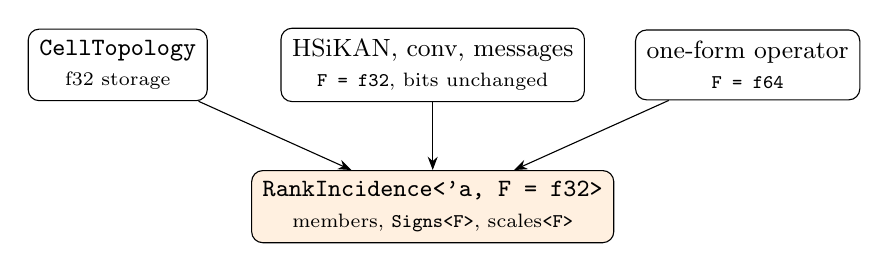
\begin{tikzpicture}[>={Stealth}, box/.style={draw, rounded corners, align=center, font=\small, inner sep=4pt}]
  \node[box, fill=orange!12] (view) at (0,0) {\texttt{RankIncidence<'a, F = f32>}\\ \scriptsize members, \texttt{Signs<F>}, scales\texttt{<F>}};
  \node[box] (topo) at (-4,1.8) {\texttt{CellTopology}\\ \scriptsize f32 storage};
  \node[box] (f32) at (0,1.8) {HSiKAN, conv, messages\\ \scriptsize \texttt{F = f32}, bits unchanged};
  \node[box] (f64) at (4,1.8) {one-form operator\\ \scriptsize \texttt{F = f64}};
  \draw[->] (topo) -- (view); \draw[->] (f32) -- (view); \draw[->] (f64) -- (view);
\end{tikzpicture}
\caption{One view, two scalars.}
\end{figure}

\end{document}
